%----------------------------------------------------------------------
\documentclass[xcolor=svgnames]{beamer} %, handout
\usetheme{lined}
\usepackage{array}
\usepackage{amsmath}
\usepackage{amssymb}
\usepackage{amsthm}
\usepackage{bbm}
\usepackage[utf8]{inputenc}
\usepackage[T1]{fontenc}
\usepackage{cmbright}   
\usepackage{times}
\usepackage{geometry}
\usepackage[spanish]{babel}
\usepackage{multicol}
\usepackage{tcolorbox}

\usepackage{algorithm2e}

%\usepackage{psfrag}
\usepackage{graphicx}
\usepackage{color}
\usepackage{floatflt}
\usepackage{fancybox}
\usepackage{tabularx}
%\usepackage[all]{xy}
\usepackage{color}
\usepackage{siunitx} % para \degree
\usepackage{mathtools}
\usepackage{cancel}
\usepackage{tikz}
\usepackage{tikz-cd}
\usetikzlibrary{arrows,matrix,positioning}


\usetikzlibrary{positioning}
\usepackage{arydshln} %poder pone lineas punteadas en matrices
\usepackage{tikz}
\usetikzlibrary{fit}
\tikzset{%
  highlight/.style={rectangle,rounded corners,fill=red!15,draw,fill opacity=0.5,thick,inner sep=0pt}
}
\newcommand{\tikzmark}[2]{\tikz[overlay,remember picture,baseline=(#1.base)] \node (#1) {#2};}
%
\newcommand{\Highlight}[1][submatrix]{%
    \tikz[overlay,remember picture]{
    \node[highlight,fit=(left.north west) (right.south east)] (#1) {};}
}



%\usepackage[most]{tcolorbox}


\theoremstyle{plain}
\newtheorem{definicion}{Definición}



\definecolor{redUnq}{rgb}{.7,.1,.1}
\definecolor{redUnq2}{rgb}{.5,.1,.3}

\mode<presentation>{
	%\usetheme{Boxes}
	%\usecolortheme[RGB={237,132,8}]{structure}
	%\usecolortheme[RGB={205,173,0}]{structure}
	\usecolortheme[RGB={100,10,10}]{structure}

	%\beamertemplateshadingbackground{SteelBlue!70}{Honeydew!10}
	%\usetheme{Warsaw}
	%\usecolortheme{default}
	\usetheme{Singapore}
	%\usetheme{Lined}
	%\usetheme[height=7mm]{Rochester} 
	\setbeamerfont{title}{shape=\bfseries,family=\rmfamily}
	%\usefonttheme[onlylarge]{structuresmallcapsserif}
	%\usefonttheme[onlysmall]{structurebold}
	\setbeamercolor{title}{fg=redUnq,bg=gray!40}
	\usefonttheme{professionalfonts}
	\setbeamercovered{highly dynamic}
	\setbeamercovered{transparent=10}
	\setbeamertemplate{navigation symbols}{}
	\colorlet{structure}{redUnq}

	\setbeamertemplate{frametitle}[default][left]
}

\definecolor{verzul}{rgb}{0, 0.5,0.5}

\renewcommand{\textbf}[1]{{\bfseries\textcolor{redUnq2}{#1}}}
\renewcommand{\emph}[1]{{\em\textcolor{redUnq2}{#1}}}

\setlength{\parindent}{0pt}
\theoremstyle{definition}
\newtheorem{ejem}{Ejemplo}
\newtheorem{defi}{Definición}
\newtheorem{ejer}{Ejercicio}
\newtheorem{prop}{Propiedad}
\newtheorem{lema}{Lema}
\newtheorem{teor}{Teorema}
\newtheorem{coro}{Corolario}

 

\newcommand{\Rset}{\mathbbmss{R}}
\newcommand{\Cset}{\mathbbmss{C}}
\newcommand{\PD}[2]{\frac{\partial #1}{\partial #2}}
\DeclareMathOperator{\tr}{tr}
\DeclareMathOperator{\adj}{adj}
\DeclareMathOperator{\rango}{rango}

\newenvironment{Boxedminipage}%
{\begin{Sbox}\begin{minipage}}%
{\end{minipage}\end{Sbox}\fbox{\TheSbox}}



\title{Métodos Numéricos - Clase 8}
  \logo{
\includegraphics[scale=0.25]{logoUnq} }
\author{Ulises Bussi- Javier Portillo}
%\institute{\scalebox{2}{\includegraphics[scale=0.1]{mdp02.jpg}}} %{Departamento de Ciencia y Tecnología\\ Universidad Nacional de Quilmes\\ }
\date{ $1^\circ$ cuatrimestre 2020} 


%%%%%%%%% Para que al comenzar una section aparezca el Contenido
%\AtBeginSection[]
%{
%  \begin{frame}
%    \frametitle{Contenidos de la Presentación}
%    \tableofcontents[currentsection]
%  \end{frame}
%}

\AtBeginSection[]
{
    \begin{frame}
        \frametitle{Derivación Numérica}
        \tableofcontents[currentsection]
    \end{frame}
}


\begin{document} 


\begin{frame} %\thispagestyle{empty}
	\titlepage
\end{frame}

\begin{frame}
\tableofcontents
\end{frame}


\section{Aproximaciones simples}

\begin{frame}
\frametitle{Derivación Numérica}

\vspace{10pt}



\begin{tcolorbox}
\textbf{¿Qué vamos a hacer?}
Muchas veces, queremos derivar una señal o conjunto de datos del que no tenemos una expresión analítica.
\end{tcolorbox} \vspace{20pt}

\pause
Las derivadas que veremos hoy serán suponiendo que el vector de variable independiente está equiespaciado



\end{frame}


\begin{frame}{Derivada hacia adelante}
	 
 Supongamos que conocemos la expresión analítica. Calculamos el polinomio de Taylor en$x_{i}$ para aproximar $f(x_{i+1})$:\vspace{-5pt}
 \only<1>{$$ f(x_{i+1}) = f(x_i) + f'(x_i) (x_{i+1}-x_i) +\frac{f''(x_i)}{2} (x_{i+1}-x_i)^2 +\dots$$}
 \only<2->{$$ f(x_{i+1}) = f(x_i) + f'(x_i) h +\frac{f''(x_i)}{2} {h^2}+\dots$$}

\visible<3->{Si despejamos $f'(x_i)$:\vspace{-3pt}

$$f'(x_i)  = \frac{f(x_{i+1}) -f(x_i)}{h} + \underbrace{\frac{f''(x_i)}{2} h +\dots}_{O(h)}$$
}

\visible<4->{\begin{tcolorbox}
\textbf{Derivada hacia adelante:}
	$$f'(x_i) = \frac{f(x_{i+1}) - f(x_i)}{h} $$\vspace{-20pt}
\end{tcolorbox}}
\end{frame}



\begin{frame}{Derivada hacia atras}
	 
 Supongamos que conocemos la expresión analítica. Calculamos el polinomio de Taylor en$x_{i}$ para aproximar $f(x_{i-1})$:\vspace{-5pt}
 \only<1>{$$ f(x_{i-1}) = f(x_i) + f'(x_i) (x_{i-1}-x_i) +\frac{f''(x_i)}{2} (x_{i-1}-x_i)^2 +\dots$$}
 \only<2->{$$ f(x_{i-1}) = f(x_i) - f'(x_i) h +\frac{f''(x_i)}{2} {h^2}+\dots$$}

\visible<3->{Si despejamos $f'(x_i)$:\vspace{-3pt}

$$f'(x_i)  = - \frac{f(x_{i-1}) -f(x_i)}{h} + \underbrace{\frac{f''(x_i)}{2} h +\dots}_{O(h)}$$
}

\visible<4->{\begin{tcolorbox}
\textbf{Derivada hacia atrás:}
	$$f'(x_i) = \frac{f(x_{i}) - f(x_{i-1})}{h} $$\vspace{-20pt}
\end{tcolorbox}}
\end{frame}


\subsection{Interpretación geométrica}


\begin{frame}{Interpretación geométrica}
  Miremos un gráfico:
  \begin{center}
      \only<1>{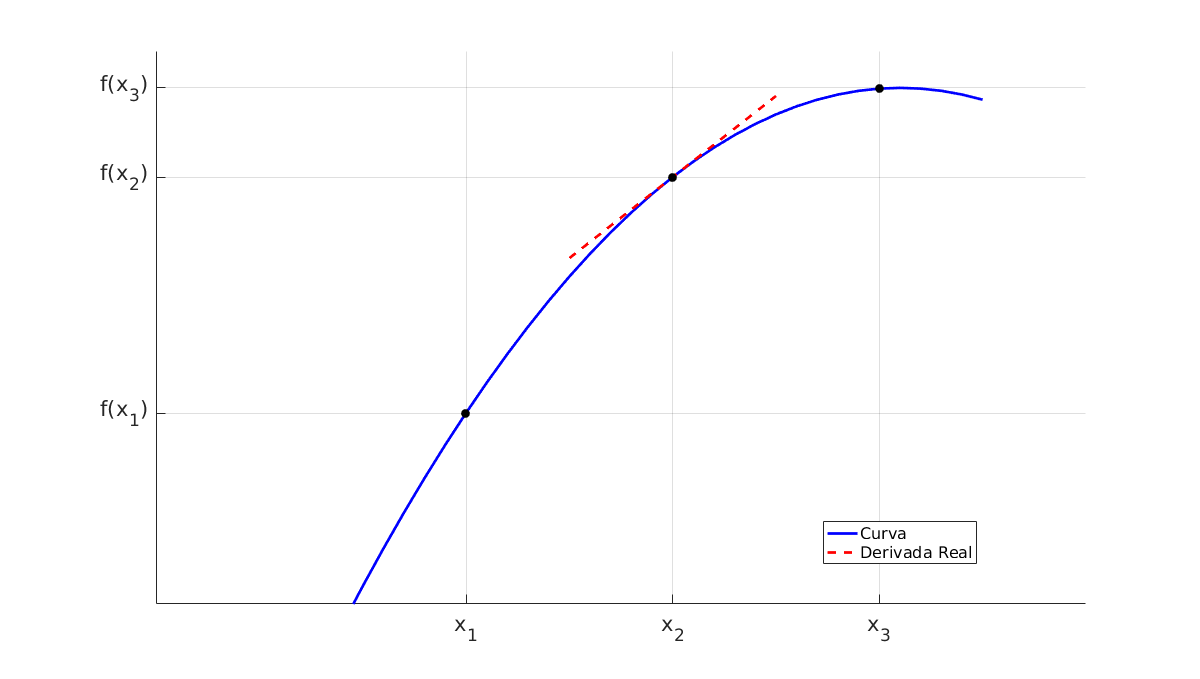
\includegraphics[width=\linewidth]{interpretacionGrafica.png} }
	  \only<2>{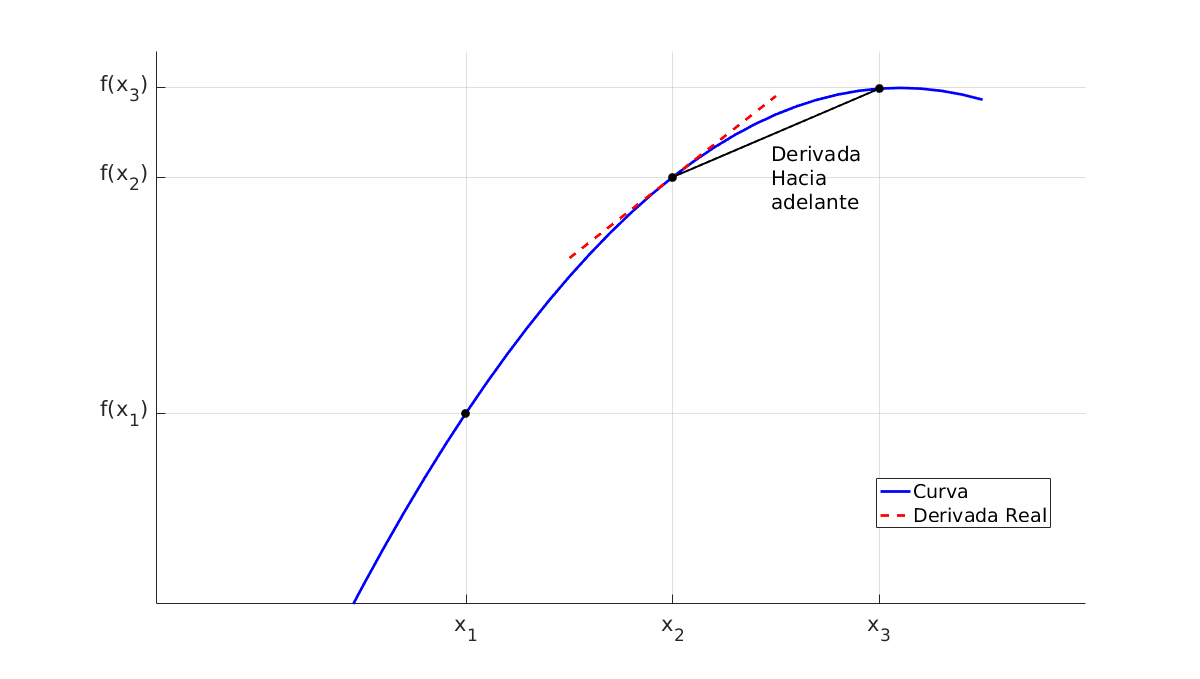
\includegraphics[width=\linewidth]{ig_forward.png} }
	  \visible<3>{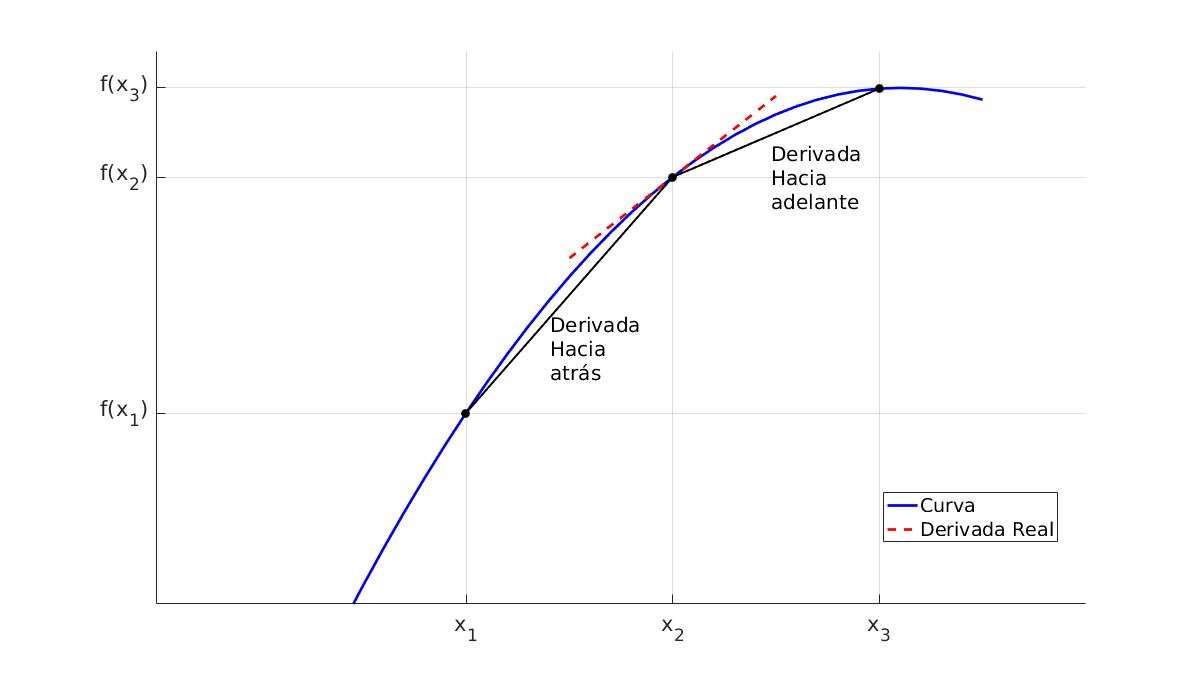
\includegraphics[width=\linewidth]{ig_backward.png} }  
  \end{center}
 
\end{frame}


\subsection{Ejemplo}

\begin{frame}
  Supongamos que tenemos $x = [1,2,3], y=[1,4,9]$ generados de la parábola
$y= x^2$ y queremos encontrar la derivada en $x=2$:

  \begin{minipage}{.55\linewidth}
	\only<1>{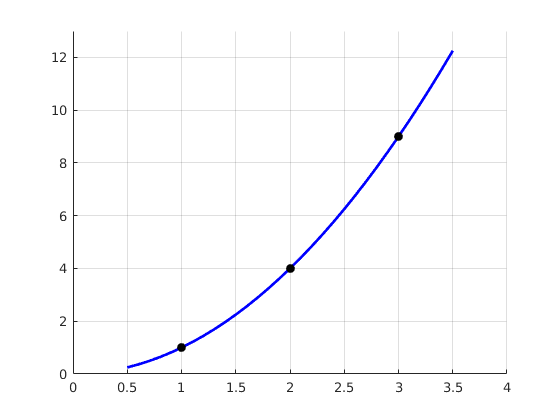
\includegraphics[width=\linewidth]{e1_0.png}}
	\only<2>{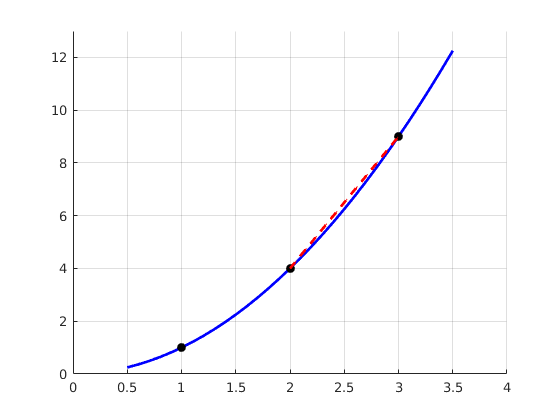
\includegraphics[width=\linewidth]{e1_1.png}}
	\only<3>{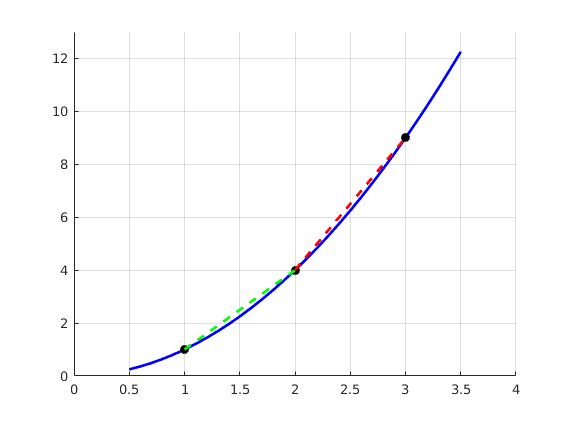
\includegraphics[width=\linewidth]{e1_2.png}}
  \end{minipage} \begin{minipage}{.41\linewidth}
	\visible<2->{  	
  	\begin{tcolorbox}
  	  \textbf{En avance:}
  	  $$ f'(x=2) \approx \frac{9-4}{3-2} =5$$
	\end{tcolorbox} }
	
	\visible<3->{
  	\begin{tcolorbox}
      \textbf{En retroceso:}
      $$ f'(x=2) \approx \frac{4-1}{2-1} =3$$
  	\end{tcolorbox} }
  \end{minipage}
\end{frame}

\subsection{Derivada Segunda}

\begin{frame}{Derivada Segunda}
  Planteamos Taylor :
  \only<1>{$$ f(x_{i+2}) = f(x_i) + f'(x_i)(x_{i+2}-x_i) +\frac{f''(x_i)}{2} (x_{i+2}-x_i)^2 +\dots$$}
  \only<2->{$$ f(x_{i+2}) = f(x_i) + f'(x_i) 2h + \frac{f''(x_i)}{2} (2h)^2 +\dots$$}
  
  \only<1>{$$ f(x_{i+1}) =  f(x_i) + f'(x_i)(x_{i+1}-x_i) +\frac{f''(x_i}{2} (x_{i+1}-x_i)^2 +\dots$$}  
  \only<2->{$$ f(x_{i+1}) =  f(x_i) + f'(x_i)(h) +\frac{f''(x_i}{2} (h)^2 +\dots$$}  
  
  \visible<3>{ tomamos la segunda, la multiplicamos x$2$ y las restamos:
  
  $$f(x_{i+2})-2f(x_{i+1}) = -f(x_i) +2 \frac{f''(x_i)}{2} h^2 +\dots$$
  
  }
\end{frame}


\begin{frame}{Derivada Segunda}  
  $$f(x_{i+2})-f(x_{i+1}) = -f(x_i) +2 \frac{f''(x_i)}{2} h^2 +\dots$$
	Despejamos $f''(x_i)$:\pause
	$$ f''(x_i) = \frac{f(x_{i+2}) -2f(x_{i+1})+f(x_{i})}{h^2} + O(h^2) $$
	\pause
	\begin{tcolorbox}  
	  \textbf{Derivada Segunda:}
	  $$ f''(x_i) = \frac{f(x_{i+2}) -2f(x_{i+1})+f(x_{i})}{h^2}$$
	\end{tcolorbox}
\end{frame}





\section{Aproximaciones superiores}


\begin{frame}{Derivada Centrada}
  Hasta acá, es sencillo el cálculo de derivadas, pero no del todo preciso.
  \pause
  
  Tomemos Taylor hacia atrás y hacia adelante:
  
  $$ f(x_{i+1})  = f(x_i) + f'(x_i) h +\frac{f''(x_i)}{2} {h^2}+\frac{f'''(x_i)}{6} {h^3}$$
  $$ f(x_{i-1}) = f(x_i) - f'(x_i) h +\frac{f''(x_i)}{2} {h^2}-\frac{f'''(x_i)}{6} {h^3}$$\pause

y las restemos: 

$$ f(x_{i+1}) -f(x_{i-1}) =2 f'(x_i) h + 2 \frac{f'''(x_i)}{6} h^3$$

\end{frame}

\begin{frame}{Derivada Centrada}
  $$ f(x_{i+1}) -f(x_{i-1}) =2 f'(x_i) h + 2 \frac{f'''(x_i)}{6} h^3$$
  Si despejamos la derivada de esta expresión:
  $$ f'(x_i) = \frac{f(x_{i+1})-f(x_{i-1})}{2 h} + \underbrace{\frac{f'''(x_i)}{6} h^2 +\dots}_{O(h^2)}$$\pause
  \begin{tcolorbox}
    \textbf{Derivada Centrada:}
    $$ f'(x_i) = \frac{f(x_{i+1})-f(x_{i-1})}{2 h} $$
  \end{tcolorbox}
  
\end{frame}

\subsection{Interpretación geométrica}

\begin{frame}{Interpretación geométrica}


  Miremos un gráfico:
  \begin{center}
      \only<1>{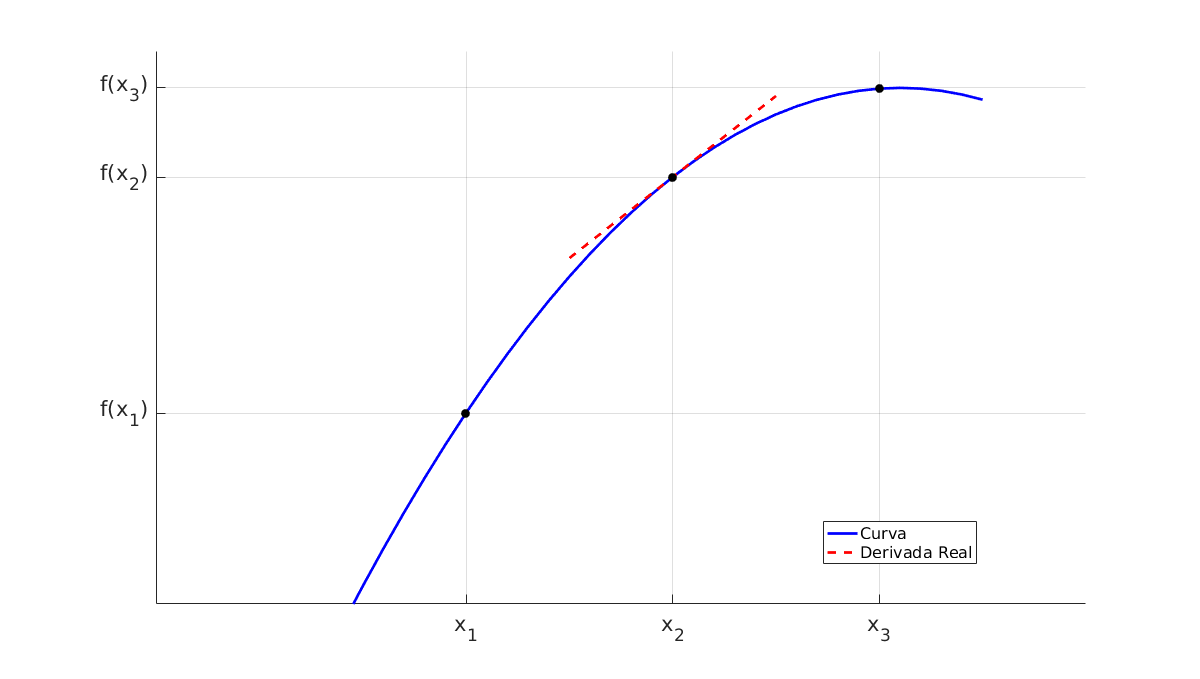
\includegraphics[width=\linewidth]{interpretacionGrafica.png} }
	  \visible<2>{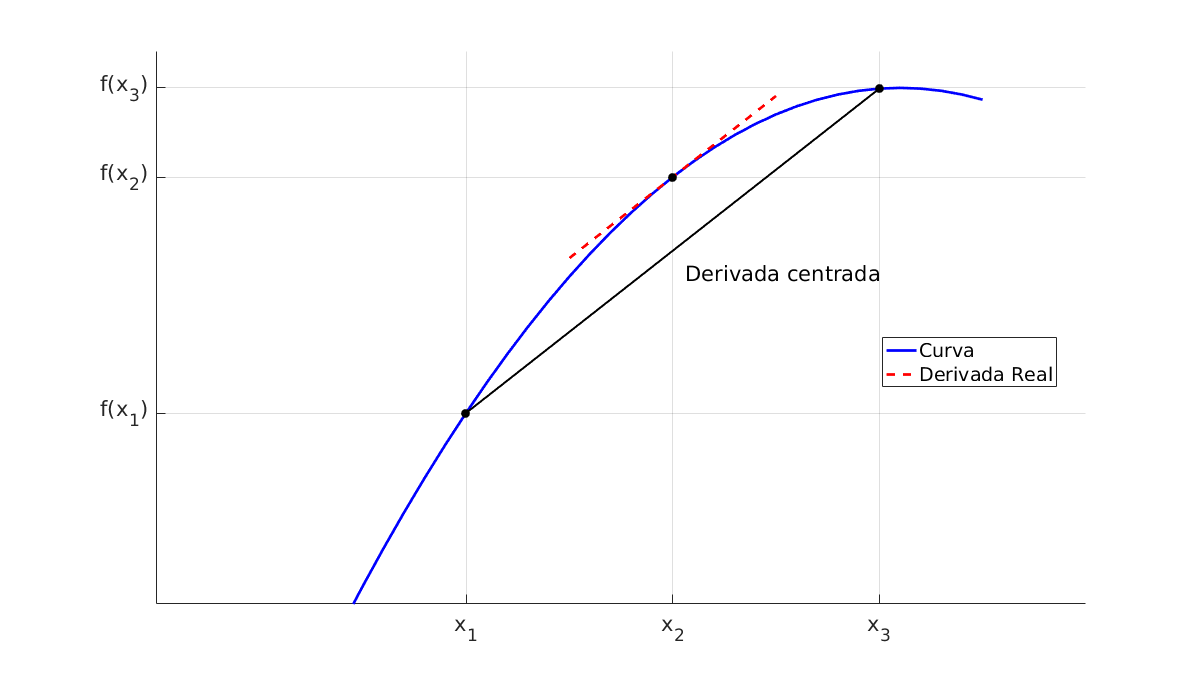
\includegraphics[width=\linewidth]{ig_center.png} }
  \end{center}
\end{frame} 



\subsection{Ejemplo}

\begin{frame}
  Supongamos que tenemos $x = [1,2,3], y=[1,4,9]$ generados de la parábola
$y= x^2$ y queremos encontrar la derivada en $x=2$:

  \begin{minipage}{.55\linewidth}
	\only<1>{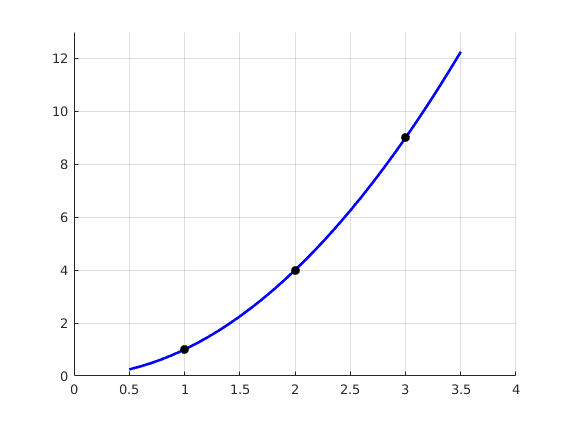
\includegraphics[width=\linewidth]{e2_0.png}}
	\only<2>{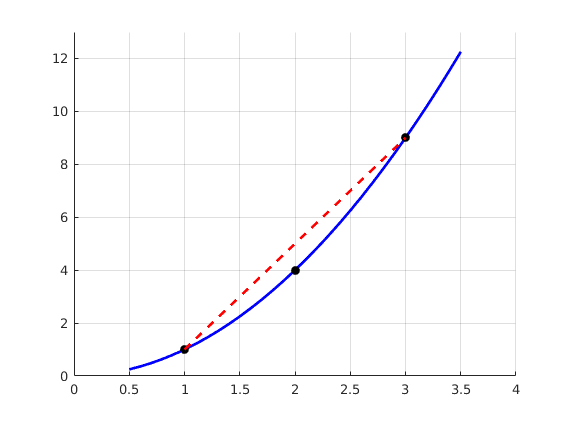
\includegraphics[width=\linewidth]{e2_1.png}}
  \end{minipage} \begin{minipage}{.41\linewidth}
	\visible<2->{  	
  	\begin{tcolorbox}
  	  \textbf{Centrada:}
  	  $$ f'(x=2) \approx \frac{9-1}{3-1} =4$$
	\end{tcolorbox} }
	
  \end{minipage}
\end{frame}


\begin{frame}{Derivada segunda centrada}
Es posible realizar un procedimiento similar para el planteo de una derivada segunda centrada cuya expresión será:\vspace{20pt}

\begin{tcolorbox}
  $$ f''(x_i) = \frac{f(x_{i+1}) -2f(x_{i})+f(x_{i-1})}{h^2}$$

\end{tcolorbox}
\end{frame}


\subsection{Aumentando la precisión}

\begin{frame}{Aumentando la precisión}
	Anteriormente vimos expresiones de la derivada primera partiendo del Taylor.\pause
	
 Donde descartamos los términos de orden 2 o superiores. Si en vez de descartar la derivada segunda la reemplazamos por la expresión que vimos antes:
  $$ f''(x_i) = \frac{f(x_{i+2}) -2f(x_{i+1})+f(x_{i})}{h^2}$$
 
  Obtendremos:
  $$f(x_{i+1}) = f(x_i) + f'(x_i) h + \frac{f(x_{i+2}) -2f(x_{i+1})+f(x_{i})}{2h^2} h^2 + \dots $$
  
  	 
\end{frame}


\begin{frame}{Aumentando la precisión}
  $$f(x_{i+1}) = f(x_i) + f'(x_i) h + \frac{f(x_{i+2}) -2f(x_{i+1})+f(x_{i})}{2h^2} h^2 + \dots $$
  
  Si despejamos la primer derivada desde aquí:\vspace{15pt} \pause
  \begin{tcolorbox}  
  
  $$ f'(x_i) = \frac{-f(x_{i+2}) +4f(x_{i+1})-3f(x_{i})}{2h} $$
  \end{tcolorbox}  
  
  
\end{frame}


\section{Inestabilidad y Amplificación de Ruido}

\begin{frame}{Inestabilidad y Amplificación de Ruido}
  Al calcular derivadas numéricamente hay que tener \textbf{Cuidado}.\vspace{15pt} \pause
  
  Si los \textbf{datos} tienen \textbf{Ruido}. \pause $\rightarrow$ Se amplifica.\vspace{15pt} \pause
  
  A veces el ruido oculta el comportamiento de la derivada.
  
\end{frame}

\begin{frame}{Amplificación de Ruido}
  Supongamos que tenemos el conjunto de datos $ x=1:.1:5, y= 50 +3\text{randn}(\text{length}(x),1)$ 
  \only<2-3>{\begin{minipage}{.45\linewidth}
	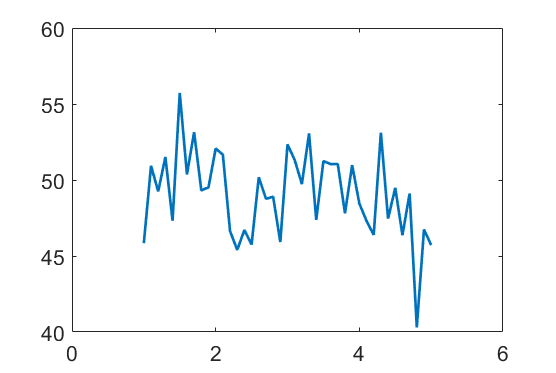
\includegraphics[width=\linewidth]{amplificacion/xy.png} 
  \end{minipage}}  \only<3>{\begin{minipage}{.45\linewidth}
	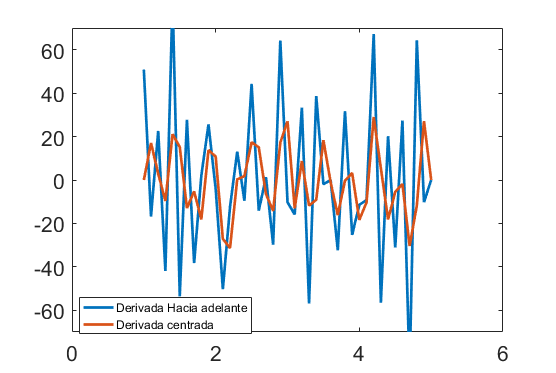
\includegraphics[width=\linewidth]{amplificacion/xy1.png} 
  \end{minipage}}
  \visible<4>{\begin{minipage}{.7\linewidth}
	  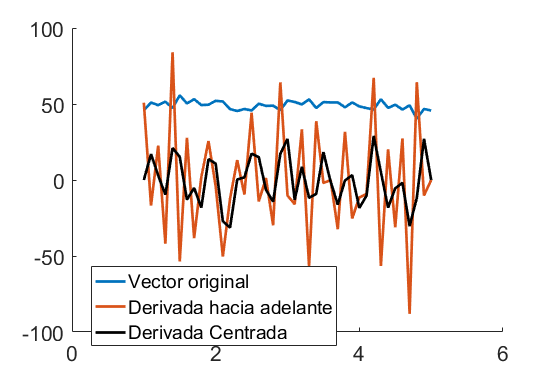
\includegraphics[width=\linewidth]{amplificacion/xyy1.png}   
  \end{minipage} \begin{minipage}{.25\linewidth}
  	$$std(y )= 2.88$$ \\
  	$$std(y'_{\text{forward}} ) = 38.41 $$\\
  	$$std(y'_{\text{center}} ) = 15.77 $$\\
  \end{minipage}    }


\end{frame}



\end{document}




%
%\subsection{Validación: Ejemplo}
%
%\begin{frame}{Validación: un Ejemplo}
%  Supongamos que tenemos el conjunto de datos:
%  \begin{minipage}{.7\linewidth}
%  \only<1-2>{  \begin{center}
%    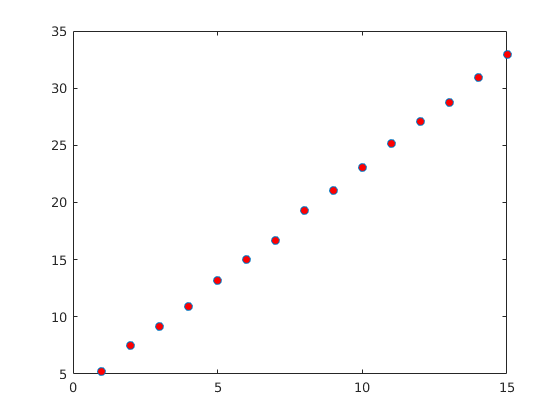
\includegraphics[width=.9\linewidth]{EjemploValidacion/dataPoints.png} 
%  \end{center}}
%    \only<3->{  \begin{center}
%    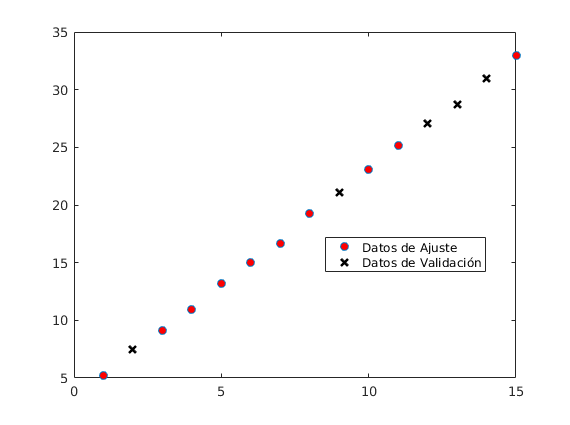
\includegraphics[width=.9\linewidth]{EjemploValidacion/dataPoints_split.png} 
%  \end{center}}
%  \end{minipage}
%  \begin{minipage}{.28\linewidth}
%	\visible<2->{Primero debemos separar nuestro set de datos}  
%  \end{minipage}
%  
%\end{frame}
%
%
%\begin{frame}{Validación: un Ejemplo}
%
%  Realizamos el ajuste con polinomios hasta de grado $4$ para ello, podemos generalizar el  problema como: $ A \underbrace{c}_{\text{coeficientes}} = b $
%donde podemos escribir
%
%\begin{minipage}{.7\linewidth}
%$$  \left[\begin{array}{*5{c}}
%    \only<1-4>{n} 			& \only<1-4>{\sum x_i}  	& \only<1-3>{\sum x_i^2}	& \only<1-2>{\sum x_i^3}	& \only<1>{\sum x_i^4}\\
%	\only<1-4>{\sum x_i}		& \only<1-4>{\sum x_i^2}	& \only<1-3>{\sum x_i^3}	& \only<1-2>{\sum x_i^4}	& \only<1>{\sum x_i^5}\\
%	\only<1-3>{\sum x_i^2} 	& \only<1-3>{\sum x_i^3}	& \only<1-3>{\sum x_i^4}	& \only<1-2>{\sum x_i^5}	& \only<1>{\sum x_i^6}\\
%    \only<1-2>{\sum x_i^3} 	& \only<1-2>{\sum x_i^4}	& \only<1-2>{\sum x_i^5}	& \only<1-2>{\sum x_i^6}	& \only<1>{\sum x_i^7}\\
%	\only<1>{\sum x_i^4}		& \only<1>{\sum x_i^5} 	& \only<1>{\sum x_i^6} 	& \only<1>{\sum x_i^7} 	& \only<1>{\sum x_i^8}
%	\end{array}\right]  \begin{bmatrix}
%	\only<1-4>{c_0}\\
%	\only<1-4>{c_1}\\
%	\only<1-3>{c_2}\\
%	\only<1-2>{c_3}\\
%	\only<1>{c_4}
%\end{bmatrix} = \begin{bmatrix}
%\only<1-4>{\sum y_i}\\
%\only<1-4>{\sum y_i x_i}\\
%\only<1-3>{\sum y_i x_i^2}\\
%\only<1-2>{\sum y_i x_i^3}\\
%\only<1>{\sum y_i x_i^4}
%\end{bmatrix}	  $$
%\end{minipage}
%\end{frame}
%
%\begin{frame}{Validación: un Ejemplo}
%Una vez hallados los coeficientes para cada caso, es posible dibujar los distintos ajustes:
%
%\begin{minipage}{.7\linewidth}
%\centering
%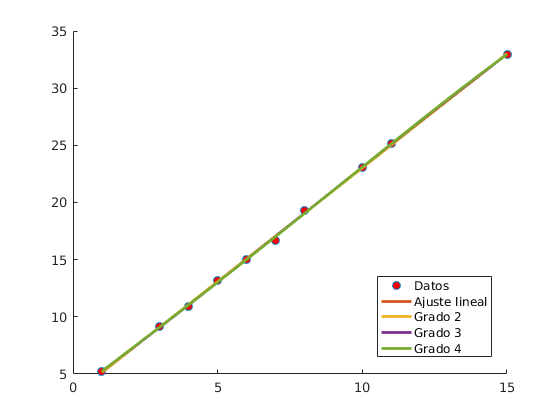
\includegraphics[width=\linewidth]{EjemploValidacion/Ajustes.png}
%
%\end{minipage}
%\begin{minipage}{.25\linewidth}
%\pause Si bien parecen todos similares miremos $r^2$
%\end{minipage}
%
%\end{frame}
%
%\begin{frame}{Validación: un Ejemplo}
%  Los coeficientes de determinación
%  \begin{center}
%  \begin{minipage}{.6\linewidth}
%    \only<1>{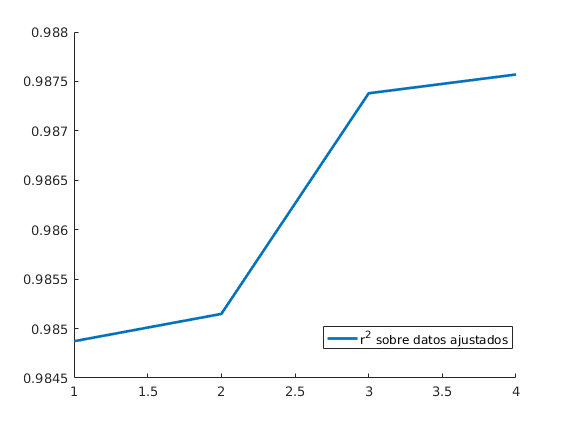
\includegraphics[width=\linewidth]{EjemploValidacion/r2_tr.png} }
%    \only<2>{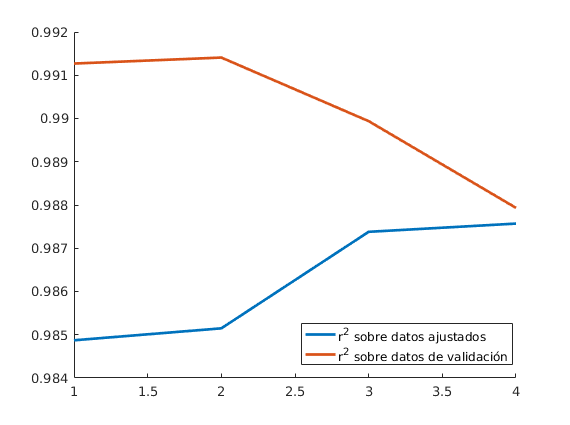
\includegraphics[width=\linewidth]{EjemploValidacion/r2_val.png} }
%  \end{minipage}
%  \end{center}\vspace{-3pt}  	
%  \pause 
%  \begin{tcolorbox}
%	\textbf{Conclusión:} El mejor ajuste parece ser el cuadrático.
%  \end{tcolorbox}
%
%\end{frame}
%
%
%\section{Interpolación}
%
%\subsection{Interpolación: Polinomios Interpoladores de Lagrange}
%
%\begin{frame}{Polinomios Interpoladores de Lagrange}
%  Proponemos interpolar 2 puntos como un promedio pesado de estos:
%  $$ f(x) =  L_1 f(x_1) + L_2 f(x_2) $$
%  \pause
%  Si la interpolación es una linea, los pesos serán una función de x:
%  $$ \begin{array}{cc}
%  L_1 = \frac{x-x_2}{x_1-x_2} \quad&\quad   L_2 = \frac{x-x_1}{x_2-x_1}
%	\end{array}   $$
%  \pause
%  Con lo que la fórmula quedará:
%  \begin{tcolorbox}	
%  	$$f(x) = \frac{x-x_2}{x_1-x_2} f(x_1) + \frac{x-x_1}{x_2-x_1} f(x_2)$$
%  \end{tcolorbox}
%
%\end{frame}
%
%\begin{frame}{Polinomios Interpoladores de Lagrange}
%  Si en cambio, queremos unir 3 puntos con una parábola, Los pesos serán:
%  $$\begin{array}{ccc}
%  L_1 = \frac{(x-x_2)(x-x_3)}{(x_1-x_2)(x_1-x_3)} & 
%  L_2 = \frac{(x-x_1)(x-x_3)}{(x_2-x_1)(x_2-x_3)} & 
%  L_3 = \frac{(x-x_1)(x-x_2)}{(x_3-x_1)(x_3-x_2)}
%  \end{array}$$
%	\pause
%  Con lo que el polinomio interpolador quedará cómo:
%  \begin{tcolorbox}
%  $$\arraycolsep=1.4pt\def\arraystretch{2.2}
%   \begin{array}{ccl}
%    f(x) &=& \frac{(x-x_2)(x-x_3)}{(x_1-x_2)(x_1-x_2)}f(x_1) +\frac{(x-x_1)(x-x_3)}{(x_2-x_1)(x_2-x_3)}f(x_2) + \\
%    & &+\frac{(x-x_1)(x-x_2)}{(x_3-x_1)(x_3-x_2)}f(x_3)  
%  \end{array}
%    $$ 
%  \end{tcolorbox}
%\end{frame}
%
%
%\begin{frame}{Polinomios Interpoladores de Lagrange}
%  Es posible generalizar los pesos, para cualquier polinomio de grado $n$:
%  $$ L_i = \prod_{j=1,j\neq i}^n \frac{x-x_j}{x_i-x_j} $$
%
%  \pause
%  El polinomio quedará:
%  \begin{tcolorbox}
%    $$ f(x) = \sum_{i=1}^n L_i(x) f(x_i) $$  
%  \end{tcolorbox}
%\end{frame}
%
%
%\subsubsection{Polinomios de Lagrange: un ejemplo}
%
%\begin{frame}{Polinomios de Lagrange: un ejemplo}
%  Supongamos que tenemos los valores $x =[1, 2, 3, 4]$  e $y= [1, 5, 3, 4]$.
%  Queremos hallar el Polinomio interpolador de Lagrange en $x = 2.5$.
%  
%  \visible<2>{  
%  \begin{center}
%  \begin{minipage}{.7\linewidth}
%	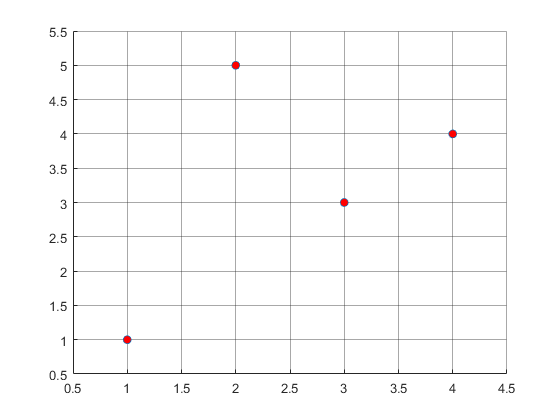
\includegraphics[width=\linewidth]{EjemploLagrange/datapts.png}  
%  \end{minipage}
%    \end{center}}
%
%\end{frame}
%
%\begin{frame}{Polinomios de Lagrange: un ejemplo}
%  Supongamos que tenemos los valores $x =[1, 2, 3, 4]$  e $y= [1, 5, 3, 4]$.
%  Queremos hallar el Polinomio interpolador de Lagrange en $x = 2.5$.
%  
%  Lo primero que hay que hacer es calcular los $L$:
%  \begin{minipage}{.45\linewidth}
%	\only<2>{$$L_1 = \frac{(x-x_2)(x-x_3)(x-x_4)}{(x_1-x_2)(x_1-x_3)(x_1-x_4)}$$}
%  	\only<3->{$$L_1 = \frac{(x-2)(x-3)(x-4)}{(1-2)(1-3)(1-4)}$$}
%	\only<4>{$$L_2 = \frac{(x-x_1)(x-x_3)(x-x_4)}{(x_2-x_1)(x_2-x_3)(x_2-x_4)}$$}
%	\only<5->{$$L_2 = \frac{(x-1)(x-3)(x-4)}{(2-1)(2-3)(2-4)}$$}
%  \end{minipage}		 \begin{minipage}{.45\linewidth}
%	\only<6>{$$L_3 = \frac{(x-x_1)(x-x_2)(x-x_4)}{(x_3-x_1)(x_3-x_2)(x_3-x_4)}$$}
%	\only<7->{$$L_3 = \frac{(x-1)(x-2)(x-4)}{(3-1)(3-2)(3-4)}$$}
%	\only<8>{$$L_4 = \frac{(x-x_1)(x-x_2)(x-x_3)}{(x_4-x_1)(x_4-x_2)(x_4-x_3)}$$}
%	\only<9->{$$L_4 = \frac{(x-1)(x-2)(x-3)}{(4-1)(4-2)(4-3)}$$}
%  \end{minipage}
%\end{frame}
%
%\begin{frame}{Polinomios de Lagrange: un ejemplo}
% 
%
%  Supongamos que tenemos los valores $x =[1, 2, 3, 4]$  e $y= [1, 5, 3, 4]$.
%  Queremos hallar el Polinomio interpolador de Lagrange en $x = 2.5$.
%  
%  Ahora debemos evaluar los $L_i$ en el punto de interés:
%  
%  \begin{minipage}{.45\linewidth}
%  \begin{tiny}
%    \only<2>{$$L_1(2,5) = \frac{(2.5-2)(2.5-3)(2.5-4)}{(1-2)(1-3)(1-4)}$$}
%	\only<3->{$$L_1(2,5) = \frac{0.5*(-0.5)*(-1.5}{(-1)*(-2)*(-3)} =-0.0625 $$}  
%	\only<4>{$$L_2(2,5) = \frac{(2.5-1)(2.5-3)(2.5-4)}{(2-1)(2-3)(2-4)}$$}
%	\only<5->{$$L_2(2,5) = \frac{1.5*(-0.5)*(-1.5}{(1)*(-1)*(-2)} = 0.5625 $$}  
%  \end{tiny}
%  \end{minipage}  \begin{minipage}{.45\linewidth}  
%  \begin{tiny}
%    \only<6>{$$L_3(2,5) = \frac{(2.5-1)(2.5-2)(2.5-4)}{(3-1)(3-2)(3-4)}$$}
%	\only<7->{$$L_3(2,5) = \frac{1.5*(0.5)*(-0.5}{(2)*(1)*(-2)} =0.5625 $$}  
%	\only<8>{$$L_4(2,5) = \frac{(2.5-1)(2.5-2)(2.5-3)}{(4-1)(4-2)(4-3)}$$}
%	\only<9->{$$L_4(2,5) = \frac{1.5*(0.5)*(-0.5}{(3)*(2)*(1)} = 0.0625 $$}  
%  \end{tiny}
%  \end{minipage}
%\end{frame}
%
%
%
%
%\begin{frame}{Polinomios de Lagrange: un ejemplo}
%  Supongamos que tenemos los valores $x =[1, 2, 3, 4]$  e $y= [1, 5, 3, 4]$.
%  Queremos hallar el Polinomio interpolador de Lagrange en $x = 2.5$.
%  
%  Por último, reemplazamos en el polinomio:
%  $$ f(2.5) = -0.0625*1 +0.5625*5 +0.5625*3-0.0625*4 $$
%  \begin{tcolorbox}
%    $$f(2.5) =  4.1875 $$
%  \end{tcolorbox}
%\end{frame}
%
%
%\begin{frame}{Polinomios de Lagrange: un ejemplo}
%  Es posible dibujar el polinomio completo si evaluamos punto a punto en matlab:
%  \begin{center}
%  \begin{minipage}{.75\linewidth}
%	  	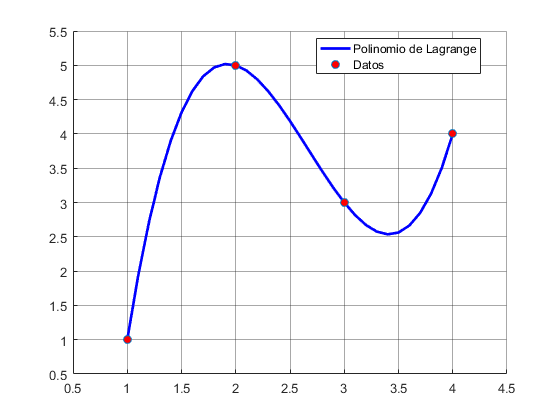
\includegraphics[width=\linewidth]{EjemploLagrange/poly.png}  
%
%  \end{minipage}
%  \end{center}
%\end{frame}
%
%
%\section{Extrapolación}
%
%\begin{frame}{Extrapolación}
%  \textbf{¿Que sucede si queremos predecir valores fuera del rango de datos?}
%  \pause
%  
%  Newton y Lagrange, sirven para interpolación pero presentan riesgos para valores externos (extrapolación). \vspace{20pt}
%  \pause
%  Tendencia es desconocida fuera del rango de datos.
%\end{frame}
%
%\subsection{Extrapolación: un Ejemplo}
%\begin{frame}{Extrapolación: un Ejemplo}
%  Supongamos que tengo los datos: \visible<2->{$x =1:.5:5$ e $y = @(x) 2*x.^2 -5*x-1 + \varepsilon$} \only<1>{\\}
%  \begin{center}
%  \begin{minipage}{.7\linewidth}
%    \only<1>{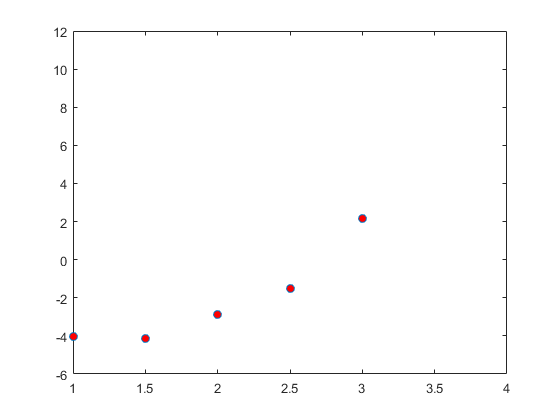
\includegraphics[width=\linewidth]{EjemploExtrapolacion/onlyPoints.png} }
%    \only<2>{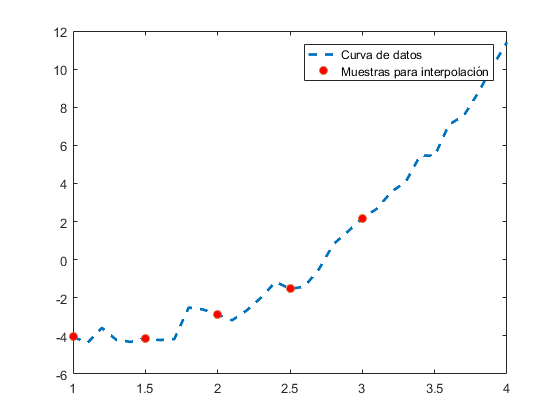
\includegraphics[width=\linewidth]{EjemploExtrapolacion/data.png} }
%    \only<3>{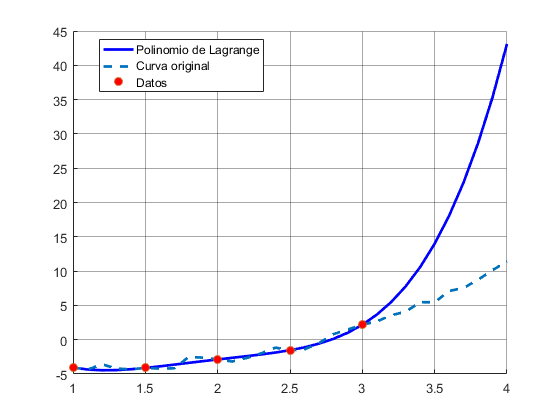
\includegraphics[width=\linewidth]{EjemploExtrapolacion/poly.png} }
%    \only<4>{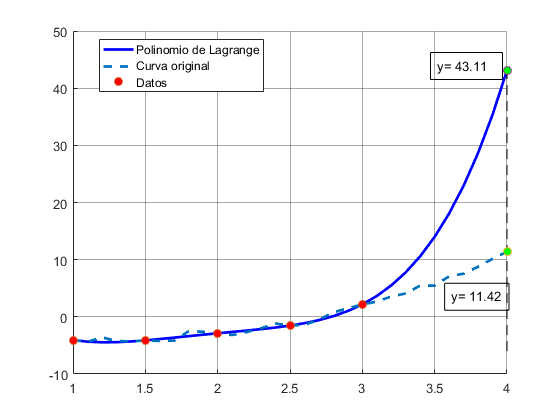
\includegraphics[width=\linewidth]{EjemploExtrapolacion/poly_vals.png} }
%  \end{minipage}
%  \end{center}  
%\end{frame}
%
%
%\section{Interpolación con Splines}
%
%\begin{frame}{Splines}
%Hasta ahora: ajustabamos polinomios de grado $n-1$ a $n$ puntos.\vspace{20pt} \pause
%
%Ahora Buscaremos aplicar funciones de orden menor.\vspace{20pt}
%
%\textbf{¿Por qué?}\vspace{10pt}\pause
%
%\begin{tcolorbox}
%\begin{center}
%  Evitar oscilaciones.
%\end{center}
%\end{tcolorbox}
%
%\end{frame}
%
%
%\begin{frame}{Splines: Lineal}
%  Propuesta: 
%  \begin{itemize}
%    \item tenemos $n$ puntos,  \pause
%    \item separamos en $n-1$ intervalos de 2 puntos. \pause
%    \item unimos los puntos de cada intervalo con rectas.\pause
%  \end{itemize}
%  
%  \begin{tcolorbox}
%    Veamos un Ejemplo
%  \end{tcolorbox}  
%\end{frame}
%
%\subsection{Spline Lineal: un ejemplo}
%
%\begin{frame}{Spline Lineal: un ejemplo}
%  $x= [1, 2, 3, 4]$\hspace{10pt}$y=[1, 5, 3, 4]$ 
%  
%  \begin{minipage}{.5\linewidth}
%    \only<1>{\includegraphics[width=\linewidth]{splines/data.png} }
%    \only<2-4>{\includegraphics[width=\linewidth]{splines/data12.png} } 
%    \only<5>{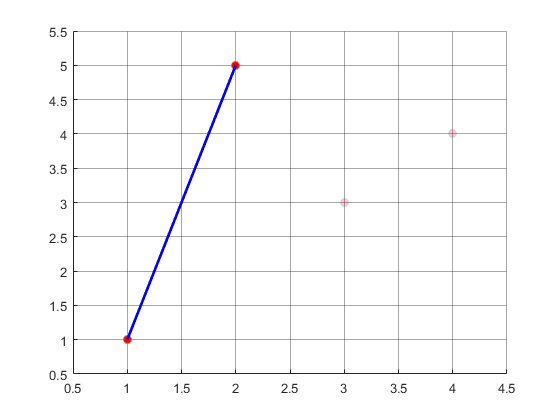
\includegraphics[width=\linewidth]{splines/data12l.png} } 
%  \end{minipage} \begin{minipage}{.45\linewidth}
%    \only<2-5>{ $s_1(x) = a_1 + b_1 (x-x_1) $} 
%    \only<3-5>{$$a_1= y_1$$}
%    \only<4-5>{$$b_1 = \frac{y_2-y_1}{x_2-x_1}$$}	  
%    \only<5>{\begin{tcolorbox}\vspace{-15pt}$$s_1(x) = 1 + 4 (x-1) $$\end{tcolorbox}} 
%  \end{minipage}
%
%\end{frame}
%
%%Frame2 ejemplo
%\begin{frame}{Spline Lineal: un ejemplo}
%  $x= [1, 2, 3, 4]$\hspace{10pt}$y=[1, 5, 3, 4]$ 
%  
%  \begin{minipage}{.5\linewidth}
%    \only<1-3>{\includegraphics[width=\linewidth]{splines/data23.png} } 
%    \only<5>{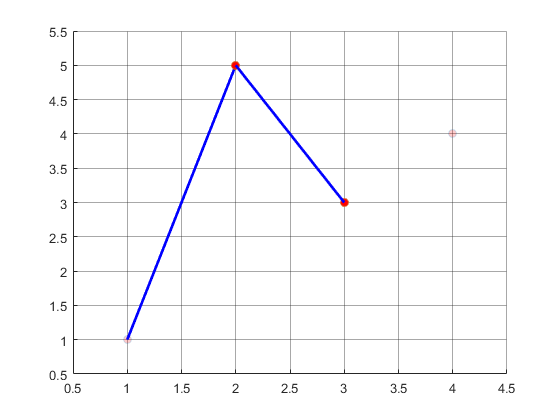
\includegraphics[width=\linewidth]{splines/data23l.png} } 
%  \end{minipage} \begin{minipage}{.45\linewidth}
%    \only<2-5>{ $s_2(x) = a_2 + b_2 (x-x_2) $} 
%    \only<3-5>{$$a_2= y_2$$}
%    \only<4-5>{$$b_2 = \frac{y_3-y_2}{x_3-x_2}$$}	  
%    \only<5>{\begin{tcolorbox}\vspace{-15pt}$$s_2(x) = 5 - 2 (x-2) $$\end{tcolorbox}} 
%  \end{minipage}
%
%\end{frame}
%
%%Frame3 ejemplo
%\begin{frame}{Spline Lineal: un ejemplo}
%  $x= [1, 2, 3, 4]$\hspace{10pt}$y=[1, 5, 3, 4]$ 
%  
%  \begin{minipage}{.5\linewidth}
%    \only<1-3>{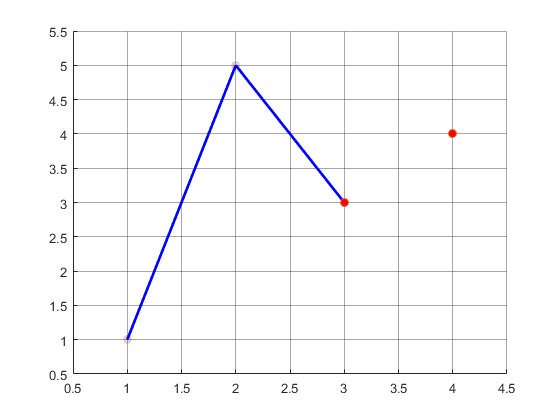
\includegraphics[width=\linewidth]{splines/data34.png} } 
%    \only<5>{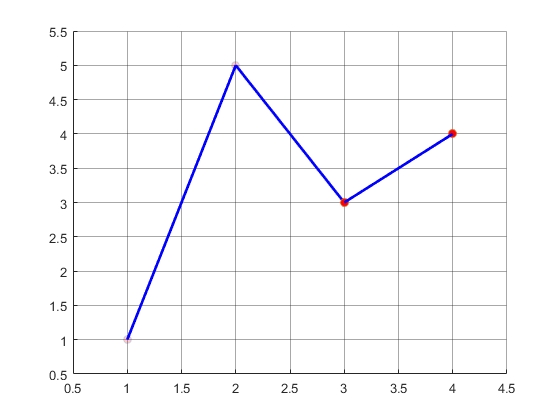
\includegraphics[width=\linewidth]{splines/data34l.png} } 
%  \end{minipage} \begin{minipage}{.45\linewidth}
%    \only<2-5>{ $s_3(x) = a_3 + b_3 (x-x_3) $} 
%    \only<3-5>{$$a_3= y_3$$}
%    \only<4-5>{$$b_3 = \frac{y_4-y_3}{x_4-x_3}$$}	  
%    \only<5>{\begin{tcolorbox}\vspace{-15pt}$$s_3(x) = 3 + 1 (x-3) $$\end{tcolorbox}} 
%  \end{minipage}
%
%\end{frame}
%
%
%%Frame4 ejemplo
%\begin{frame}{Spline Lineal: un ejemplo}
%  $x= [1, 2, 3, 4]$\hspace{10pt}$y=[1, 5, 3, 4]$ 
%  \begin{center}
%    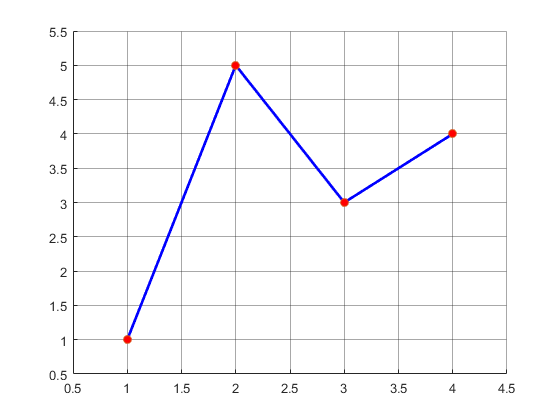
\includegraphics[width=.45\linewidth]{splines/splineLin.png}  
%  \end{center}
%  \begin{tcolorbox}
%	$$S(x) = \left\{
%	\begin{array}{cc}
%	  1 + 4(x-1) ,& \text{si } x \in [1,2) \\
%	  5 - 2(x-2) ,& \text{si } x \in [2,3) \\
%	  3 + (x-3)  ,& \text{si } x \in [3,4] \\
%	\end{array} \right.$$		
%  \end{tcolorbox}
%
%\end{frame}
%
%\subsection{Spline Lineal}
%\begin{frame}{Spline Lineal: resumiendo}
%	\begin{itemize}
%	\item Tomamos los $n$ puntos y dividimos en $n-1$ intervalos.\pause
%	\item Calculamos la recta que va en cada intervalo:\pause
%	$$s_i(x) = a_i + b_i(x-x_i)  $$\pause
%	$$\boxed{a_i = y_i} \quad \boxed{b_i = \frac{y_{i+1}-y_i}{x_{i+1}-x_i}}$$\pause
%	\item Creamos la función partida $S(x)$.
%	\end{itemize}
%
%\end{frame}
%
%
%
%\subsection{Spline Cuadrático}
%
%\begin{frame}{Spline Cuadrático}
%Ahora propondremos ajustar funciones cuadráticas a los pares de puntos. Para esto agregaremos una condición:\vspace{15pt}\pause
%
%\textbf{La derivada en cada punto debe ser continua}\vspace{15pt} \pause
%
%Nuestros $s_i$ tendrán la forma
%
%$$ s_i(x) = a_i +b_i(x-x_i) + c_i(x-x_i)^2$$ \pause
%
%Es inmediato ver que $s_i(x_i) = a_i = y_i$.
%
%\end{frame}
%
%
%\begin{frame}{Spline Cuadrático}
%  \only<1-2>{Para asegurar la continuidad hasta la primer derivada tomemos $s_i$ y $s_{i+1}$:
%  $$\begin{array}{cclllll}
%     s_i(x) &=& y_i &+& b_i(x-x_i) &+& c_i(x-x_i)^2\\
%     s_{i+1}(x) &=& y_{i+1} &+& b_{i+1}(x-x_{i+1}) &+& c_{i+1}(x-x_{i+1})^2
%\end{array}   $$ }
%  \only<2->{Tendremos que: $s_i(x_{i+1}) = s_{i+1} (x_{i+1})$ (continuidad)
%  $$y_i + b_i(x_{i+1}-x_{i})+ c_i(x_{i+1}-x_{i})^2 = y_{i+1} +0 + 0$$}
%  \only<3->{Tendremos que $s'_i(x_{i+1}) = s'_{i+1} (x_{i+1})$ (derivada continua)
%  $$ b_i + 2c_i \underbrace{(x_{i+1}-x_{i})}_{h_i} = b_{i+1} + 0$$}
%  
%\end{frame}
%
%\begin{frame}{Spline Cuadrático}
%  Vamos a escribir las ecuaciones, supongamos que son 4 puntos:\pause
%  $$\begin{array}{ccc}
%    y_i +{\color{red}b_1} h_1 + {\color{red}c_1} h_1^2 &=& y_2 \\
%    {\color{red}b_1} + 2{\color{red}c_1} h_1 &=& {\color{red}b_2} \\
%    y_2 + {\color{red}b_2} h_2 + {\color{red}c_2} h_2^2 &=& y_3 \\
%    {\color{red}b_2} + 2{\color{red}c_2} h_2 &=& {\color{red}b_3} \\
%    y_3 + {\color{red}b_3} h_3 + {\color{red}c_3} h_3^2 &=& y_4 \\
%%%    {\color{red}b_3} + 2{\color{red}c_3} h_3 &=& {\color{red}b_4} \\
%  \end{array}$$\pause
%  \begin{minipage}{.45\linewidth}
%	  \begin{tcolorbox}
%	     Tenemos 6 incógnitas y 5 ecuaciones!
%  	  \end{tcolorbox}  
%  \end{minipage}\pause \hspace{15pt}$\rightarrow$\hspace{15pt}  Pidamos $c_1=0$
%
%\end{frame}
%
%
%\subsubsection{Spline Cuadrático: un ejemplo}
%
%\begin{frame}{Spline Cuadrático: un ejemplo}
%   $x= [1, 2, 3, 4]$\hspace{10pt}$y=[1, 5, 3, 4]$ 
%  
%  \begin{minipage}{.5\linewidth}
%    \only<1>{\includegraphics[width=\linewidth]{splineCuad/data.png} } 
%    \only<2-5>{\includegraphics[width=\linewidth]{splineCuad/data12.png} } 
%    \only<6>{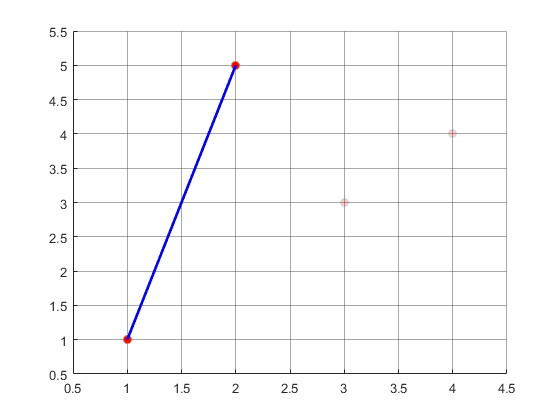
\includegraphics[width=\linewidth]{splineCuad/data12l.png} } 
%  \end{minipage} \begin{minipage}{.45\linewidth}
%    \only<2-6>{ $s_1(x) = a_1 + b_1 (x-x_1) + c_1 (x-x_1)^2$} 
%    \only<3-6>{$$a_1= y_1= 1$$}
%    \only<4-6>{$$c_1 = 0$$}
%    \only<4>{$$y_1 + b_1 h = y_2$$}	  
%    \only<5-6>{$$b_1= \frac{y_2-y_1}{h} $$}
%    \only<6>{\begin{tcolorbox}\vspace{-15pt}$$s_1(x) = 1 + 4 (x-1) $$\end{tcolorbox}} 
%  \end{minipage}
%\end{frame}
%
%%frame 2
%\begin{frame}{Spline Cuadrático: un ejemplo}
%   $x= [1, 2, 3, 4]$\hspace{10pt}$y=[1, 5, 3, 4]$ 
%  
%  \begin{minipage}{.5\linewidth}
%    \only<1-5>{\includegraphics[width=\linewidth]{splineCuad/data23.png} } 
%    \only<6>{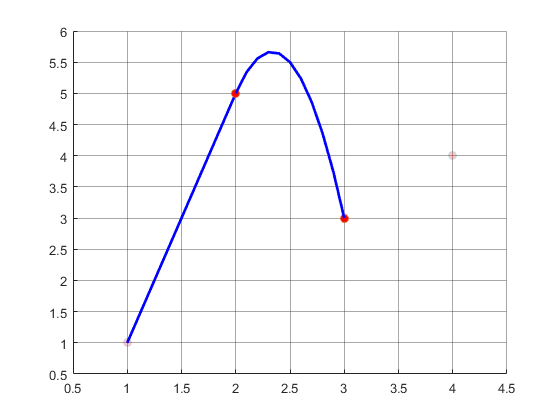
\includegraphics[width=\linewidth]{splineCuad/data23l.png} } 
%  \end{minipage} \begin{minipage}{.45\linewidth}
%    \only<2-6>{ $s_2(x) = a_2 + b_2 (x-x_2) + c_2 (x-x_2)^2$} 
%    \only<3-6>{$$a_2= y_2= 5$$}
%    \only<4-6>{$$b_2 = b_1+ 2c_1 h_1 = 4$$}
%    \only<4>{$$c_2 = \frac{y_3-y_2 -b_2*h_2}{h_2^2}$$}	  
%    \only<5-6>{$$c_2= \frac{-2-4}{1} = -6 $$}
%    \only<6>{\begin{tcolorbox}\footnotesize \vspace{-15pt}$$s_2(x) = 5 + 4 (x-2) - 6(x-2)^2 $$\end{tcolorbox}} 
%  \end{minipage}
%\end{frame}
%
%%frame 3
%\begin{frame}{Spline Cuadrático: un ejemplo}
%   $x= [1, 2, 3, 4]$\hspace{10pt}$y=[1, 5, 3, 4]$ 
%  
%  \begin{minipage}{.5\linewidth}
%    \only<1-5>{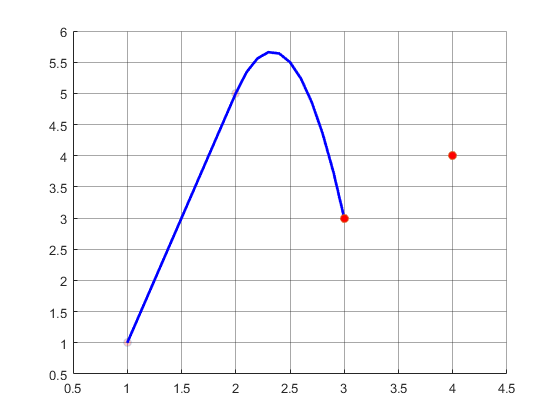
\includegraphics[width=\linewidth]{splineCuad/data34.png} } 
%    \only<6>{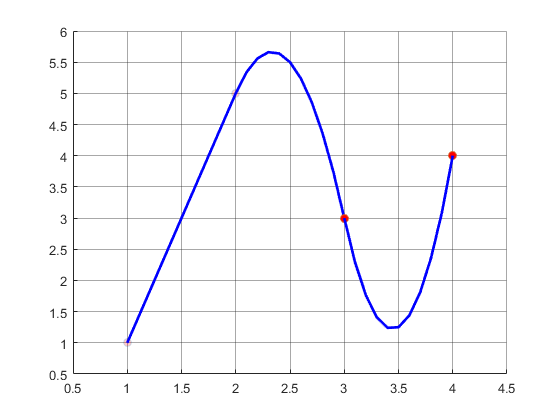
\includegraphics[width=\linewidth]{splineCuad/data34l.png} } 
%  \end{minipage} \begin{minipage}{.45\linewidth}
%    \only<2-6>{ $s_3(x) = a_3 + b_3 (x-x_3) + c_3 (x-x_3)^2$} 
%    \only<3-6>{$$a_3= y_3= 3$$}
%    \only<4-6>{$$b_3 = b_2+ 2c_2 h_2 = -8$$}
%    \only<4>{$$c_3 = \frac{y_4-y_3 -b_3*h_3}{h_3^2}$$}	  
%    \only<5-6>{$$c_3= \frac{1+8}{1} = 9 $$}
%    \only<6>{\begin{tcolorbox}\footnotesize \vspace{-15pt}$$s_3(x) = 3  -8 (x-3) +9 (x-3)^2 $$\end{tcolorbox}} 
%  \end{minipage}
%\end{frame}
%
%
%
%%Frame4 ejemplo
%\begin{frame}{Spline Cuadrático: un ejemplo}
%  $x= [1, 2, 3, 4]$\hspace{10pt}$y=[1, 5, 3, 4]$ 
%    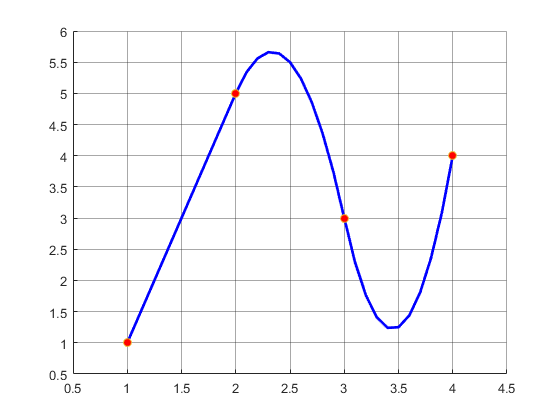
\includegraphics[width=.45\linewidth]{splineCuad/splineLin.png}  
%
%  \begin{tcolorbox}
%	$$S(x) = \left\{
%	\begin{array}{cc}
%	  1 + 4(x-1) ,& \text{si } x \in [1,2) \\
%	  5 +4(x-2)-6(x-2)^2 ,& \text{si } x \in [2,3) \\
%	  3 - 8(x-3)+9(x-3)^2  ,& \text{si } x \in [3,4] \\
%	\end{array} \right.$$		
%  \end{tcolorbox}
%\end{frame}
%
%\subsubsection{Spline Cuadrático: resumiendo}
%\begin{frame}{Spline Cuadrático: resumiendo}
%	\begin{itemize}
%	\item Tomamos los $n$ puntos y dividimos en $n-1$ intervalos.\pause
%	\item Calculamos la parabola que va en cada intervalo:\pause
%	$$s_i(x) = a_i + b_i(x-x_i) + c_i(x-x_i)^2  $$\pause
%	$$\boxed{a_i = y_i} \quad \boxed{b_i = b_{i-1}+2c_{i-1}h_{i-1}}$$
%	$$\boxed{c_i = \frac{y_{i+1}-y_i-b_ih_i}{h_i^2}} $$\pause
%	\item Creamos la función partida $S(x)$.
%	\end{itemize}
%
%\end{frame}
%
%
%%
%%\subsection{Spline Cúbico}
%%
%%\begin{frame}{Spline Cúbico}
%% Si propondremos ajustar funciones cúbicas necesitamos una condición adiciona:\vspace{15pt}\pause
%%
%%\textbf{La derivada segunda en cada punto debe ser continua}\vspace{15pt} \pause
%%
%%Nuestros $s_i$ tendrán la forma
%%
%%$$ s_i(x) = a_i +b_i(x-x_i) + c_i(x-x_i)^2+ d_i(x-x_i)^3$$ \pause
%%
%%Es inmediato ver que $s_i(x_i) = a_i = y_i$.
%%
%%\end{frame}
%%
%%\begin{frame}{Spline Cúbico}
%%	Tomemos $S_i$ y sus derivadas:
%%	
%%	$$s_i(x)= y_i+b_i(x-x_i)+c_i(x-x_i)^2+d_i(x-x_i)^3$$
%%	$$s'_i(x)= b_i+2c_i(x-x_i)+3d_i(x-x_i)^2$$
%%	$$s''_i(x)= 2c_i+6d_i(x-x_i)$$
%%
%%\end{frame}
%%
%%
%%\begin{frame}{Spline Cúbico}
%%  Igualemos $s''_i(x_{i+1}) =s''_{i+1}(x_{i+1})$ (segunda derivada igual):
%%  $$ 2{\color{red}c_i} +6 {\color{red}d_i}\underbrace{(x_{i+1}-x_i)}_{h_i} =2{\color{red}c_{i+1}} + 0$$
%%  Lo mismo para $s'_i(x_{i+1}) =s'_{i+1}(x_{i+1})$ (primer derivada igual):
%%  $$ {\color{red}b_i} + 2{\color{red}c_i}h_i +3{\color{red}d_i}h_i^2 = {\color{red}b_{i+1}}$$
%%  Por último con $s_i(x_{i+1}) = s_{i+1}(x_{i+1})$:
%%  $$ y_i + {\color{red}b_i}h_i +{\color{red}c_i}h_i^2 +{\color{red}d_i}h_i^3 = y_{i+1}$$
%%\end{frame}
%%








